\chapter{Deep Learning}

\section{Overview}

An auspicious field of machine learning is deep learning. It tries to solve optimisation and generalisation problems by the use of artificial neural networks (ANN). Neural networks have the ability to learn non-linear and complex relationships in data. The network is called neural, because the millions of connections between single nodes are mimicking the architecture of the human brain. A neural network consists of neurons grouped together in so-called layers. These neurons are connected to other neurons in the previous and next layer. The shape of a neural network is very versatile. It needs to contain at least an input and an output layer. With the use of hidden layers, the network can be trained on recognising patterns in the data set. Unlike the input or output layer, the hidden layers are invisible for the developer and act like a black box \cite{nn}.

\begin{figure}[!ht]
    \centering
    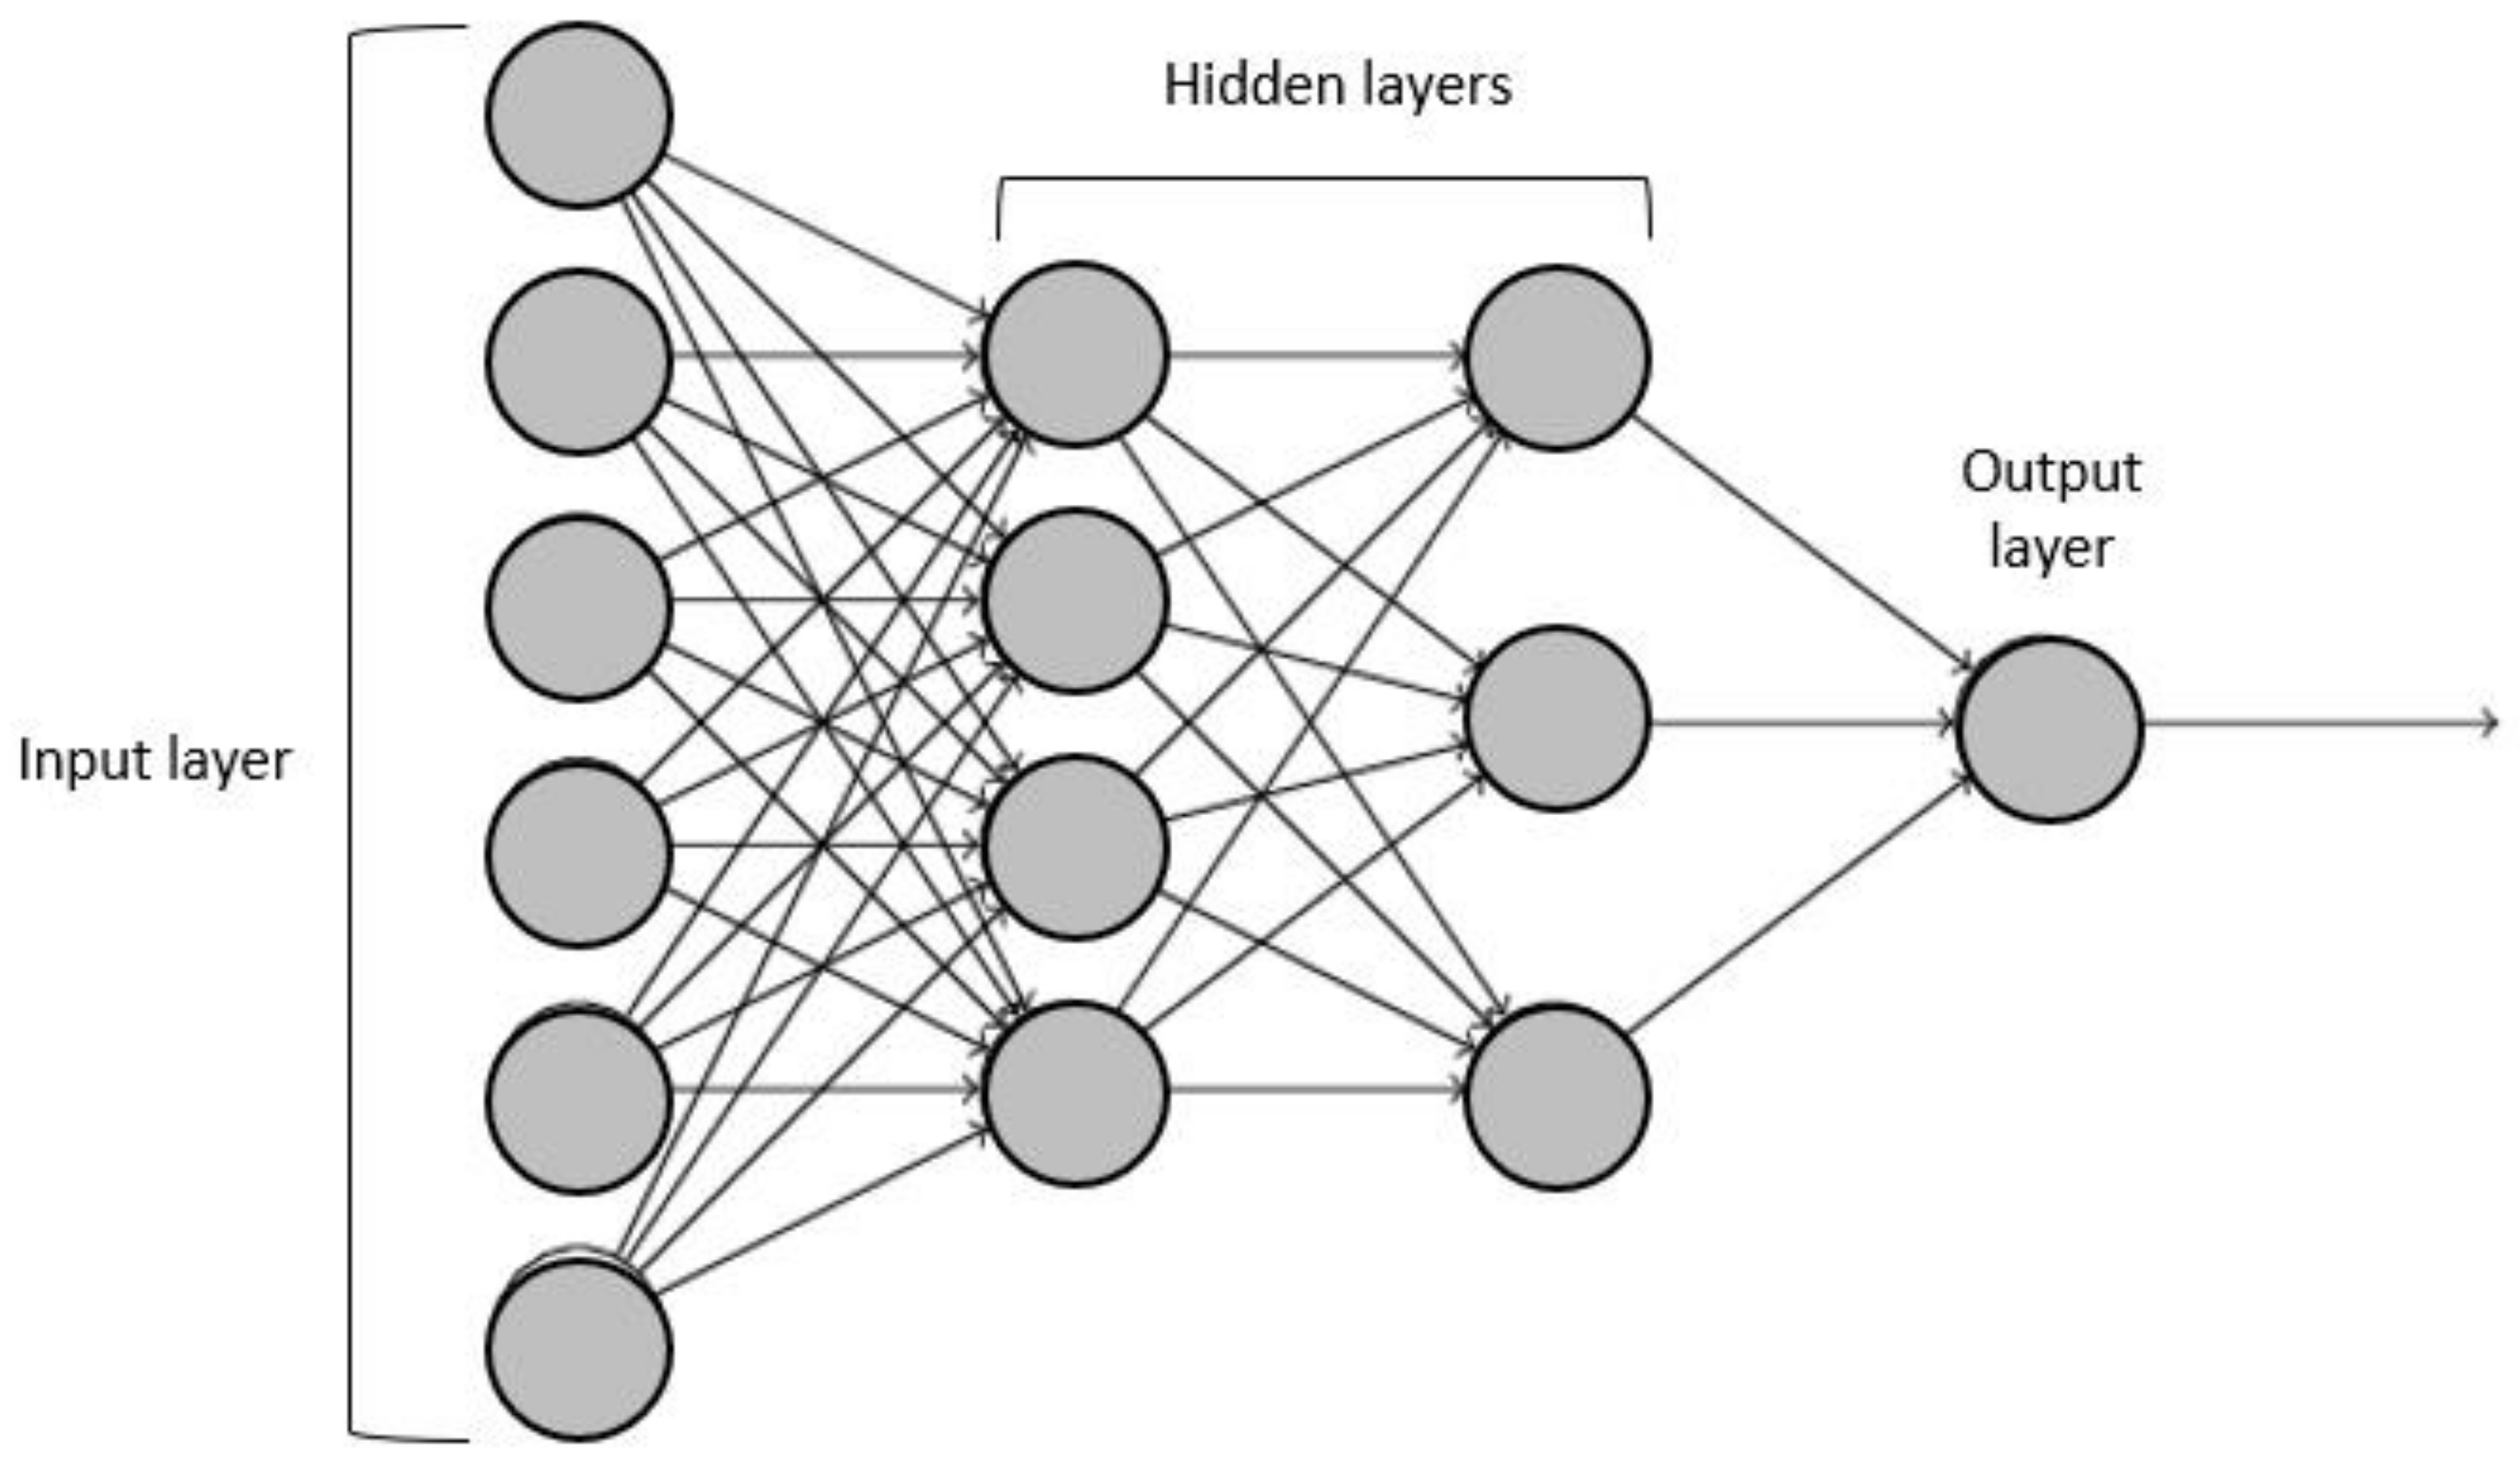
\includegraphics[scale=0.6]{neural-network}
    \caption{Architecture of a neural network}
    \label{fig:nn}
\end{figure}

The output layer represents the predictions a neural network makes. This might be a single neuron for a binary classification or multiple neurons, each representing a different class to predict. A network classifying cat an dog images may have a single output neuron where $0$ represents a cat and $1$ a dog picture.

\subsection{Functionality}

The basic idea behind neural networks goes back to 1958. Even today's neurons are based on the \emph{perceptron}, developed by Frank Rosenblatt at Cornell University \cite{wiki06}. A single perceptron (or neuron) contains several inputs $x$, which are each multiplied by an independent weight $w$. The output of a perceptron is the sum of all weighted inputs and the bias $\Theta$\footnote{Allows you to modify the outcome by shifting the activation function in a certain direction} processed by an output function called \emph{activation function} \cite{perc17}.

\begin{figure}[!ht]
    \centering
    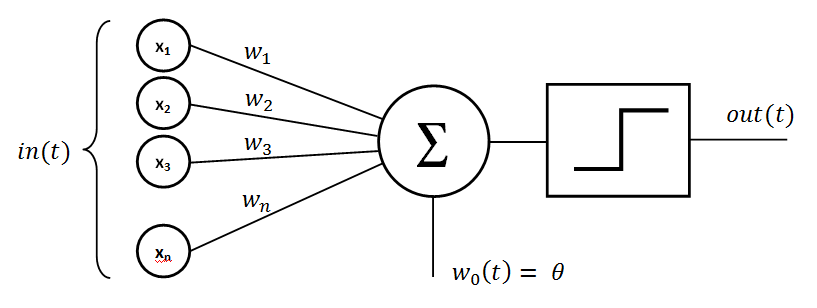
\includegraphics[scale=0.5]{perceptron}
    \caption{Parts of a perceptron}
    \label{fig:perceptron}
\end{figure}

By training with a vast amount of samples, a deep learning model tries to understand a problem and creates generalised solutions for it. Therefore the neural network needs labelled training data. This means that the data scientist needs to tell the network the answer for every samples passing through the network. Considering the image classification example from above, every cat and dog picture needs to be labelled as such. Neural networks rely on two basic concepts called \emph{feed-forward} and \emph{backpropagation}.

\subsubsection{Feed-forward}

The feed-forward process of a neural network passes the input values through the hidden layers to the output layer. Each neuron sends its output to the connected neurons in the following layer. Every connection has a weight which is multiplied by the outgoing value before being used as an input of the next neuron. As seen in figure \ref{fig:perceptron}, the output gets calculated by the activation function. There are several functions applicable and it's the developer's choice which one to use \cite{nn}. Processing every output according to the weighted input values is a very simple mathematical operation\footnote{It is basically a matrix multiplication}. The vast amount of connections is thereby responsible for the sometimes very long training duration.

\subsubsection{Backpropagation}

After the feed-forward phase, the output of a neural network needs to be compared against the actual correct output. The difference between these two values is called \emph{error}. Because a neural network is initialised with random weights, the error between prediction and truth value is typically very high at beginning.

Backpropagation is the process of iterating through the network in reverse order from the end to the beginning and adjusting the weights of every connection in the right direction to minimise the previously calculated error \cite{nn}.

A training of a neural network consists of multiple feed-forward and backpropagation phases, using a different input sample for every run. The backpropagation can be done after every sample\footnote{This type of training is called online learning and is very memory efficient}. On the other hand it's often useful if multiple samples are grouped to batches and the backpropagation is only done after the whole batch is passed through the network\footnote{This training is called batch learning and is more robust against bad input data}. This type of learning averages the final weight adjustment and the neural network doesn't get too much affected by a single noisy sample.

\subsection{Applications}

Neural networks are widely used in almost every industry branch including health services, electronics, finance, or even military. They can identify cancerous cells, predict stock market prices or translate texts into any other language. Most applications seem to be very easy for a human being to solve, but are quite difficult for a machine to understand.

Natural language processing offers a large variety of tasks where deep learning can be used too. Except from NER there exists machine translation, part-of-speech tagging, spell checking or text classification \cite{olga17}.

\section{Splitting your Data}

A neural network should learn complex patterns instead of the data itself. This problem is called \emph{overfitting} and will be discussed later in this section. To make generalised predictions, it is essential to split your data into different subsets. It's crucial that these subsets cover all aspects of your data evenly. Imagine a model for recognising cat and dog images which hasn't seen a single cat image at training phase. Such model would poorly perform when tested with a picture of a kitten.

The \emph{training set} is usually the largest subset, including all samples used for fitting the model to a specific problem. In many cases it contains about 80\% or more of the overall data. The model learns from this subset in multiple iterations, called epochs \cite{shah17}.

The \emph{validation set} refers to a small amount of data inside the training set. It is being used for evaluating the model at training phase mostly unbiased. It is mostly unbiased, because the model adjusts its parameters according to the validation with this data set. Therefore you can say, that the model (indirectly) learns from the validation set as well. Jason Brownlee wrote a great article about the differences of test and validation sets \cite{brown17}. I use the validation set to stop the training before overfitting occurs.

A final evaluation is done by the \emph{test set}. This data has to be new to the model to make valid statements about the model's performance. The performance on the test set should be slightly worse than on the training or validation set due to values it hasn't seen before \cite{shah17}.

\subsection{Used Data Sets}

The data of the final deep learning approach is split into the three parts mentioned above. As seen in figure \ref{fig:datasets}, the train-test split is about 80-20\% which is a common ratio. The same test set is being used for evaluating the baseline model as well.

\begin{figure}[!ht]
    \centering
    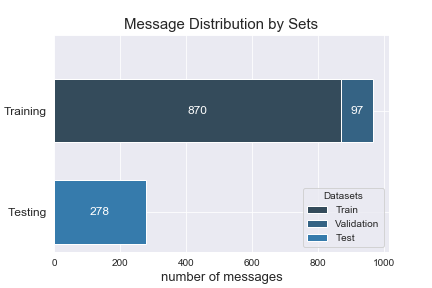
\includegraphics[scale=0.6]{plot-datasets}
    \caption{Different data sets}
    \label{fig:datasets}
\end{figure}

\subsection{Overfitting}
\label{chap:overfitting}

Overfitting occurs when a model starts to memorise the training data rather than learning from the signal. This happens when the model is trained with too many epochs. The error on the training set is continually decreasing, but starts increasing on previously unseen data. As visible in figure \ref{fig:overfit}, overfitting starts at epoch 18. The red line symbolises the point for early stopping where the data scientist would normally end the training. The error on the training set is still decreasing after every epoch.

\begin{figure}[!ht]
    \centering
    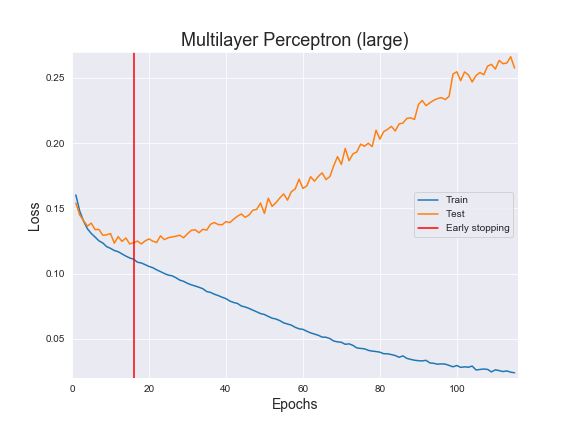
\includegraphics[scale=0.4]{plot-overfit}
    \caption{Example of an overfitted model}
    \label{fig:overfit}
\end{figure}

To avoid overfitting, a deep learning model should use at least two different data sets to validate the training process and stop before overfitting occurs. Another useful method is to reduce the parameter space so the model doesn't have the capability of learning noisy data. In deep learning there is the possibility of adding dropouts. This technique randomly disables neurons in all layers while training. Neighbouring neurons now need to compensate the dropped out neurons. This boosts generalisation of the network because neurons doesn't get specialised for single features \cite{drop14}. But in the end, the best option against overfitting is still using a much larger amount of training data which makes it harder for the network to memorise.

\section{Defining the Model}

There exist countless ways how a neural network can be designed. A well-constructed deep learning model shouldn't only rely on a single token to make its predictions. Especially in NLP the context is fundamental for making suitable predictions. By context the neighbouring words are meant. The input of a neural network has to be numerical. Otherwise the multiplication with the weights wouldn't be possible. Another fact is, that the input needs to be the same size for every sample, so you couldn't simply pass sentences inside the network without preprocessing. A clever method to pass sequences of tokens into a network is the \emph{sliding window} technique, described in the next section.

\subsection{Sliding Windows}
\label{chap:sliding-window}

Due to different lengths of the text samples, the input layer of the neural network cannot rely on the number of words in the corpus. It has to be consistent throughout the whole training and validation process. One possible solution is to adjust the input dimension to the size of the longest sentence in the corpus, but this would wastefully bloat the network's parameter space. Needless to say that this enormous structure is only used by the longest text and is an overhead for all other input values. Another possibility is to use the \verb|pad_sequences()|\footnote{more information at https://keras.io/preprocessing/sequence} function of \emph{Keras} which simply trims sentences to a specific length. Unfortunately many tokens at the end of texts will get cut off.

Therefore the sliding window functionality comes in very handy. It creates multiple windows with of a defined length but with different tokens. Every token of a text is at least once present in a window. Listing \ref{code:sliding-window} shows how these slices are generated.

Table \ref{tbl:sliding-window} illustrates the \verb|sliding_window()| function with an example. The colourized cell indicates the current token which the network should predict. This single sentence results in eight windows. The sliding window technique duplicates the input data thus the original 967 sentences are split into 70354 windows of size 9.

\begin{table}[ht!]
    \centering
    \begin{tabular}{|c|c|c|c|c|c|c|c|c|}
        \hline
        \verb|i| & \multicolumn{7}{c|}{\textbf{Sliding Window}} \\ [0.5ex]
        \hline
        1 &  &  &  & \cellcolor[HTML]{eaeaf2} Bond & drinks & his & vodka \\ [0.5ex]
        \hline
        2 &  &  & Bond & \cellcolor[HTML]{eaeaf2} drinks & his & vodka & martini \\ [0.5ex]
        \hline
        3 &  & Bond & drinks & \cellcolor[HTML]{eaeaf2} his & vodka & martini & shaken, \\ [0.5ex]
        \hline
        4 & Bond & drinks & his & \cellcolor[HTML]{eaeaf2} vodka & martini & shaken, & not \\ [0.5ex]
        \hline
        5 & drinks & his & vodka & \cellcolor[HTML]{eaeaf2} martini & shaken, & not & stirred. \\ [0.5ex]
        \hline
        6 & his & vodka & martini & \cellcolor[HTML]{eaeaf2} shaken, & not & stirred. & \\ [0.5ex]
        \hline
        7 & vodka & martini & shaken, & \cellcolor[HTML]{eaeaf2} not & stirred. &  & \\ [0.5ex]
        \hline
        8 & martini & shaken, & not & \cellcolor[HTML]{eaeaf2} stirred. &  &  & \\ [0.5ex]
        \hline
    \end{tabular}
    \caption{Sliding windows of size 7}
    \label{tbl:sliding-window}
\end{table}

\subsection{Using Keras Tokenizer}
\label{chap:tokenizer}

The input into a neural network has to be numeric. Therefore a very simple solution is to map every word to an unique ID. The \emph{Keras tokenizer} creates an ID for every distinctive word in the training data. As seen in table \ref{tbl:keras-tokenizer} the IDs are ranked by their frequency in the text. The words \emph{to} and \emph{be} are more frequent than the rest so they have got a lower ID.

\begin{table}[ht!]
    \centering
    \begin{tabular}{|l|c|c|c|c|c|c|c|c|c|c|}
        \hline
        \textbf{Original} & To & be, & or & not & to & be, & that & is & the & question. \\
        \hline
        \textbf{Tokenized} & 2 & 3 & 4 & 5 & 2 & 3 & 6 & 7 & 8 & 9 \\
        \hline
    \end{tabular}
    \caption{Example output of the Keras tokenizer}
    \label{tbl:keras-tokenizer}
\end{table}

The first ID is reserved for a special token called \emph{OOV} (out-of-vocabulary). You have to fit the tokenizer on a given text which may not contain the same tokens than the test set. Every word which the \emph{tokenizer} hasn't seen before gets labelled as \emph{OOV}. Consider listing \ref{code:keras-tokenizer} to see how the tokenizer is being used.

\subsubsection{Disadvantages}

The main downside of using a tokenizer is that the IDs doesn't provide any additional information about the token itself. For example the Swiss German word \emph{Velo}, which means bicycle, is probably more frequently used in the corpus than the German version \emph{Fahrrad}. These two words share a very strong similarity but this relation is invisible when using IDs. Another disadvantage is, that higher IDs might have higher weights than lower ones \cite{nurz18}. Therefore \emph{embeddings} should be used as described in section \ref{chap:embd}.

\subsection{Output Layer}

To classify all tokens into the three classes \emph{O}, \emph{PER}, and \emph{LOC}, several solutions are applicable. Rather than getting a single neuron as output I chose to use three output neurons where all are representing a single class. The \emph{softmax} function (\ref{math:softmax}) can be used to parse every output value to a percentage. It simply calculates the weighted input $wx$ summarized with the bias $b$ of a given neuron and divides it by the sum of all output neurons \cite{soft}.

\begin{equation}
    \label{math:softmax}
    P(y=j | x) = \frac{e^{(w_jx+b_j)}}{\sum_{k \in K} e^{(w_kx+b_k)}}
\end{equation}

Another popular activation function for a single output layer is called \emph{Sigmoid}. The s-shaped function returns values from $0$ to $1$, very useful for representing probabilities. Because the \emph{Sigmoid} is a little harder to compute than other functions, \emph{ReLU} is currently the most used activation function in neural networks. Consider the references for more information \cite{act17}.

\subsection{Enlarging the Parameter Space}

\begin{figure}[!ht]
    \begin{subfigure}{0.5\textwidth}
        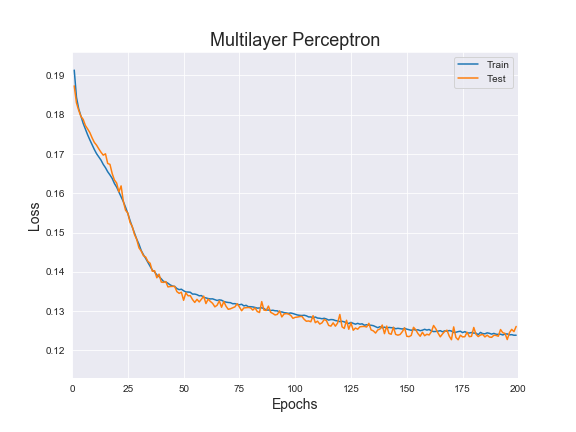
\includegraphics[scale=0.3]{plot-mlp-small}
        \caption{Initial (323 parameters)}
        \label{fig:plot-mlp-small}
    \end{subfigure}
    \begin{subfigure}{0.5\textwidth}
        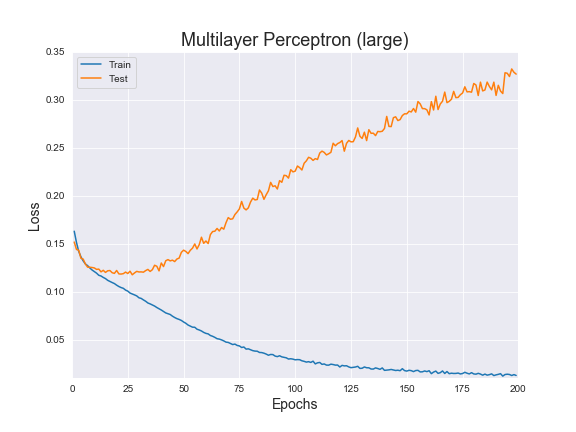
\includegraphics[scale=0.3]{plot-mlp-large}
        \caption{Enlarged (69'123 parameters)}
        \label{fig:plot-mlp-large}
    \end{subfigure}
    \caption{Performance comparison between different parameter spaces}
\end{figure}

As visible in figure \ref{fig:plot-mlp-small}, even after more than 150 epochs the smaller model continuously learns. But it doesn't learn very well and only makes tiny steps forward. The model's 323 parameters aren't enough to recognise addresses. After increasing its size to more than 69'000 parameters, the model is finally able to learn addresses as well. Figure \ref{fig:plot-mlp-large} visualises very good, that the enlarged model starts to overfit after more than 25 epochs. But the enlarged model might be too big, so that it doesn't have the urge to generalise at all. Additionally a smaller model benefits from shorter training times.

\subsection{Implementing Class Weights}

Due to the very imbalanced data set, the model mostly learns how to detect outside tokens rather than named entities. This procedure isn't efficient. With the use of class weights, you can tell the model that named entities should have more impact in adjusting the weights of the neural network \cite{imb18}. \emph{Scikit-learn} offers a clever function to calculate weights according to frequency of the entities\footnote{The function $compute\_class\_weight()$ in the $sklearn.utils$ package}. For a balanced training, the \emph{PER} entities should be weighted 26 times more than outside tokens. For locations it's even more than 63 times. Surprisingly the use of class weights doesn't affect the model's performance at all.

\subsection{Word Embeddings}
\label{chap:embd}

Word embeddings represent words as high-dimensional vectors with real numbers. They allow words with similar meaning to have a similar representation in the vector space \cite{emb18}. As pictured in figure \ref{fig:embeddings}, words of a similar meaning like locations or vehicles can be grouped together.

\begin{figure}[!ht]
    \centering
    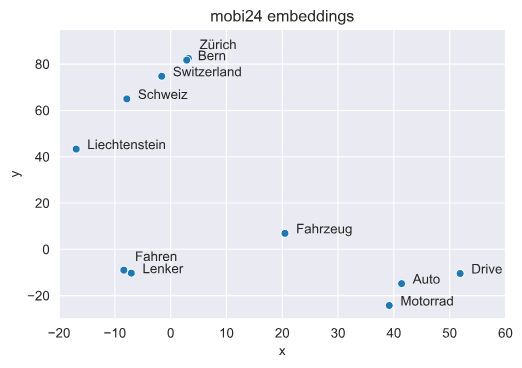
\includegraphics[scale=0.4]{embeddings}
    \caption{Visualisation of word embeddings}
    \label{fig:embeddings}
\end{figure}

These embeddings are built with Gensim's \emph{word2vec}\footnote{See \url{https://radimrehurek.com/gensim/models/word2vec.html} for more information} model on the Mobi24 data. Though the relatively small vocabulary of about 14500 tokens, there is enough context in the data so that cities like \emph{Bern} and \emph{Zurich} are displayed very similar. The embeddings are computed with 20 dimensions. More dimensions allow words to be described more precisely but need much more computation time. The vectors have been reduced to only two dimensions\footnote{Dimensionality reduction has been done with TSNE of the scikit-learn package} to display them. Consider \ref{code:embeddings} to see how embeddings can be created by the use of \emph{Gensim}.

Word embeddings are often independent of the underlying data source. Therefore it is usual that pre-calculated embeddings of famous corpora can be used. The final embeddings of the neural model are based on the wikipedia corpus, have 300 dimensions and have been re-trained with the Mobi24 data.

The performance of a model with embeddings is much better than with the use of the meaningless tokenizer IDs (see \ref{chap:tokenizer}). With the custom created Mobi24 embeddings, which only have 20 dimensions and a very small vocabulary of 14'500 tokens, the \emph{f1-score} reaches over 80\%. Combined with the vast vocabulary of Wikipedia, these embeddings are responsible for the highest achieved scoring during this bachelor thesis.

\section{Performance}
\label{chap:deep-performance}

The final deep learning approach uses a subset of the fine tuning options mentioned in the sections above. Class weights should allow the network to basically learn on the relevant parts, but seem to be worthless in this specific case. Embeddings have replaced the keras tokenizer, which give the network a basic understanding of word meanings. The final model only needs about five epochs to train before it starts overfitting.

\begin{figure}[!ht]
    \centering
    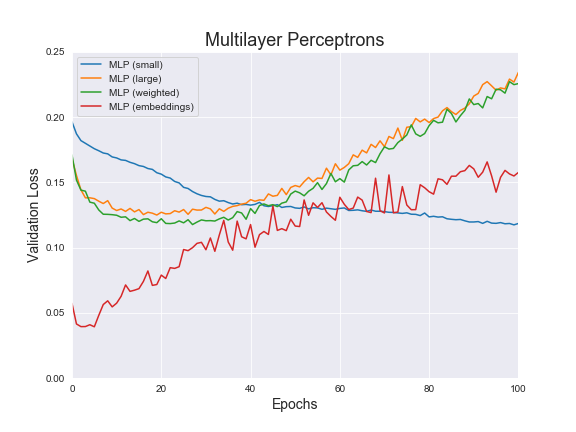
\includegraphics[scale=0.4]{plot-comparisons}
    \caption{Comparison of all deep learning approaches}
    \label{fig:plot-comparisons}
\end{figure}

Compared to the performance of the previous deep learning approaches (consider figure \ref{fig:plot-comparisons}), the embeddings deliver the largest performance increase. A larger parameter space allows the model to learn locations as well, whereas the original smaller network isn't able to do so. But a too large parameter space is also bad. Then the network can possibly memorise every sample in the first run and will build up neurons only representing a specific sample \cite{drop14}.

If we have a look at table \ref{tbl:perf-mlp}, there can be found several surprising findings. First it is unexpected that the use of class weights only slightly improves the model's performance. On the final model there is as good as no improvement visible. In theory, class weights should be a reasonable way against imbalanced data sets \cite{imb18}. It is astonishing as well, that the generated embeddings increase the \emph{f1-score} from 35\% to more than 80\% although the underlying vocabulary doesn't contain many of the tokens in the test set. With the final embeddings, the German Wikipedia corpus retrained with the Mobi24 data, the model reaches a \emph{f1-score} of more than \textbf{95.3\%}.

\subsection{Remaining Errors}

Tested with the separate test set of 278 messages, there are still some errors left. But as visible in the confusion matrix \ref{tbl:final-errors}, the number of falsie classified words is only about \textbf{0.528\%}.

\begin{table}[ht!]
    \centering
    \begin{tabular}{|c|c|c|}
        \hline
        & \multicolumn{2}{c|}{\textbf{True value}} \\
        \hline
        \textbf{Prediction} & \cellcolor[HTML]{eaeaf2} named-entity & \cellcolor[HTML]{eaeaf2} outside \\
        \hline
        \cellcolor[HTML]{eaeaf2} named-entity & 940 & 56 \\
        \hline
        \cellcolor[HTML]{eaeaf2} outside & 49 & 18826 \\
        \hline
    \end{tabular}
    \caption{Confusion matrix of the final NN}
    \label{tbl:final-errors}
\end{table}

If we have a closer look at the 56 \emph{false positives} - remember, the tokens wrongly predicted as named-entities - we can see some patterns. The Swiss law states, that some legal structures like sole proprietorships need to include the family name in their business name. Due to this, the model sometimes classifies parts of organisations as names. Additionally, it struggles with names including parenthesis at the beginning. And it's not that surprising, that email addresses including names are classified as such. Another good example for word ambiguity is the \emph{Skoda Oktavia}, where the second part is also recognised as name.

On the other hand, there are \emph{false negatives} like \emph{Biqkaj, Carisch, Coradi,} or \emph{Tschirky} which are not classified as named entities. To be honest, these names doesn't sound very familiar and are even for humans hard to guess when given without context. More confusing is the fact, that countries like \emph{Thailand, Tansania, Malaysia, Italien, Schweiz} and cities like \emph{Karlsruhe, Dortmund,} and \emph{Bienne} are not identified as locations.

\begin{figure}[!ht]
    \centering
    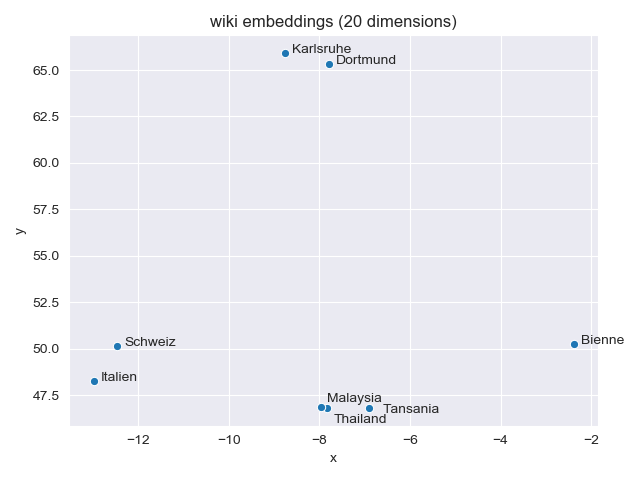
\includegraphics[scale=0.4]{embeddings-issue}
    \caption{Visualisation of the false negative tokens}
    \label{fig:embd-issue}
\end{figure}

Figure \ref{fig:embd-issue} shows very well, that the vector representations of these terms can be easily clustered. You can make a distinction between the two Asian countries and Europe. Even more impressive is the proximity of \emph{Karlsruhe} and \emph{Germany}. Pay attention to the TSNE\footnote{t-Distributed stochastic neighbor embedding} dimensionality reduction, which has been done, due to save computational time, with only 10'000 vectors and not the full 703'000, the Wikipedia embeddings would consist of. The resulting groups would be even more accurate if they would have been used. Therefore it's uncertain why these terms doesn't get recognised as NE. 

\section{Conclusion}

Working with neural networks can be painful. You don't have any insights in this black box of hidden layers. Adjusting parameters like the batch size\footnote{Number of samples fed forward before the weights get adjusted}, parameter space\footnote{Defined by the number of layers and their amount of neurons}, or class weights have no measurable impact on this named-entity recognition with the given training and test data. Due to the randomised initialisation of the weights, there are slightly different KPIs after every training. This makes it almost impossible to make concrete statements about an adjustment.

Although all the downsides mentioned above, there are several deep learning paradigms which demonstrate the performance benefits. Clean data is essential for the model to train on. Additionally the model's performance should be validated with two different, yet unseen data sets. Using the validation set for performance adjustments while training, the test set helps to compare the trained model to different solutions. The probably most useful enhancement is the switch from tokenised IDs to word vectors.

Finally, the deep learning model beats the baseline approach by far. Compared to the baseline's \emph{f1-score} of 78.6\%, the neural network reaches up to \textbf{95.3\%}. The high \emph{f1-score} gets reflected by the values for precision and recall. This is a very satisfying result in relation to the limited time span of this project and the very little data\footnote{About 1000 email messages are not the epitome of big data} available for training.
